%!TEX root = ../main.tex

\chapter{Preliminary project}
\noindent
The project is made by three main components: \ac{VR} APP, backend, Web \ac{UI}. This chapter will talk about them.
\section{The user experience}
\paragraph{VR APP}
The user experience in the \ac{VR} app will be designed to be intuitive, there will be two types of users: professors and students.
Professors will have the ability to create a virtual classroom. Students can join these rooms by entering a unique code provided to them. Once inside, the professor will guide the lecture by showcasing 3D models of different hearts.
They can manipulate these models by moving, resizing, and using a laser pointer to highlight specific areas of interest. 
\paragraph{WEB UI}
The Web app will let the professor to upload any OBJ models needed for the lecture by a simple form, and the web app will allow to view 3D models.

\section{The VR APP}
\noindent
This section will explain the main choices behind the \ac{VR} APP
\paragraph{The development environment:} 
There are three main way to develop on the Meta Quest 2:

\begin{itemize}
  \item \textbf{Native:} By using native \ac{API} that Meta provides for the \ac{HMD}.
  \item \textbf{Unity:} Is a famous game engine principally used for lightweight video games, It is pretty functional and easy to use, its programming language is \texttt{C\#}. 
  \item \textbf{Unreal Engine:} Is a famous game engine used for big games, its performance is the best in the market, it uses \texttt{C++} and a graphical programming language called Blueprint.
\end{itemize}
\noindent
As we said in the non-functional requirements we will use a game engine, I have opted for \ac{UE} because of its performance, the 3D models that will use are complex (\textasciitilde1-10MBytes in size),
so it will be used for its performance, also it has a lot of tools for multiplayer and a good documentation other than a big community of developers.

\section{Unreal Engine}
\noindent
Made by Epic Games, the project was born for the video game Unreal,
now it is one of the best engines that power a lot of important video games and 3D animation. 
For this project it will use the 5.2.1 version because at the time of writing this thesis for the best compatibility with the \ac{HMD}. 
The main reason for this upgrade was for faster building time and more advanced \ac{API} of Meta. 

\paragraph{The fundamentals:}
\ac{UE} has a 3D preview mode that lets the user set the various 3D objects in the scene.
In unreal a scene is called "Level", each element in a level is called "Actor", Actors are made by multiple components.\\
Each element of unreal can be built with a proprietary system called Blueprint, a visual programming interface, or via \texttt{C++}, or by combining them.
Principally Blueprint can make the development of the project faster and easier at the cost of performance, \texttt{C++} performs better, and it has a bigger range of tools.
So It is important to combine both languages for having the best performance and flexibility in the project.\\
Like a lot of game engines, \ac{UE} tries to render many frames as much as possible, each cycle of rendering is called tick.\\
It's important that long actions must be asynchronous with respect to the game ticks, and if something must be a runner in the so-called "game thread", it must be as fast as possible so that the frame rate does not drop to a certain level.\\
Another important component is the player controller, this is the instance of a player inside a level, a player controller can possess a pawn actor or a character actor.


\paragraph{External library:}
One challenge for this application is having a correctly multiplayer session between \ac{HMD}, unfortunately \ac{UE} does not provide a \texttt{VRpawn} that has multiplayer functionality.
For having a faster developing experience, a library called VRexpansion\footnote{\url{https://vreue4.com/}} will help the development, the library is open source under MIT licensing.
The main useful components are:
\begin{itemize}
  \item \textbf{VRcharacter:} a character for \ac{VR} games, all its components can be replicated in a multiplayer session.
  \item \textbf{Grippable Interface:}  interface that can enable actors or static meshes to be gripped by the \ac{HMD} components. It also can be replicated in a multiplayer session.
\end{itemize}

\paragraph{Events:}
Events are what start the execution of code inside a Blueprint. Each blueprint have its own standard event, they depend on the object, the basic ones are:
\begin{itemize}
  \item \textbf{Begin Play:} runs one time when the actor is spawned (this is not a constructor).
  \item \textbf{On tick:} runs on every game tick.
\end{itemize}
\noindent
We can also create custom events with Blueprint or \texttt{C++}, they can be triggered whenever we want, they can also be replicated in clients in multiplayer sessions. 
Like functions, events can have inputs but not outputs.

\paragraph{Multiplayer:}
\ac{UE} just supports a client-server configuration for managing multiplayer sessions, it has two main implementations: Stand-Alone server and listening server.\\
A Stand-Alone server consists in having a server that emulates the gaming session, it requires a server powerful enough to run the basic function of the game event if it does not need to render it.\\
A Listening Server does not need a Stand-Alone server, simply one device acts not only as a client but also as a server. Normally client-server is the best in performance and latency, but because this software is simple, the listening server is the right implementation.\\
For making a good multiplayer we have some blueprints that can help with the synchronization of the data: 

\begin{itemize}
  \item \textbf{Game Mode:} runned only inside the server, as it is called it provides the rules how the game should work, it is important for the login and log out of the players.
  \item \textbf{Game state:} it represents the state of the game, all \ac{HMD} has one, but it is always replicated by the server.
  \item \textbf{Player controller:} runned in every \ac{HMD}, it represents the player using the \ac{HMD}.
  \item \textbf{Player state:} it has all the data of a player like the username, its replicated.
\end{itemize}
\noindent
An important feature for synchronize events between client and server are \ac{RPCs}, \ac{RPCs} are events of actors that can per reproduce in multiple device at once by following one of these rules:
\begin{itemize}
  \item \textbf{Client:} The \ac{RPCs} are executed on the owning client connection for this actor.
  \item \textbf{Server:} The \ac{RPCs} are executed on the server, it must be called from the client that owns this actor.
  \item \textbf{Multicast:} The \ac{RPCs} are executed on the server and all currently connected clients the actor is relevant for, Multicast \ac{RPCs} are designed to be called from the server, but can be called from clients. A Multicast \ac{RPCs} called from a client only executes locally.
\end{itemize}

\section{Network Infrastructure}
\noindent
The Network Infrastructure [fig:\ref{fig:NetworkSchema}] it is simple, a server will be hosted in the IT department of the hospital that will host the \ac{REST} server for managing 3D Models and multiplayer sessions,
and in the same server will host via NodeJS the Web Portal for managing the 3DModels.
The multiplayer itself will be manage by the host \ac{HMD}

\begin{figure}[h]
  \centering
  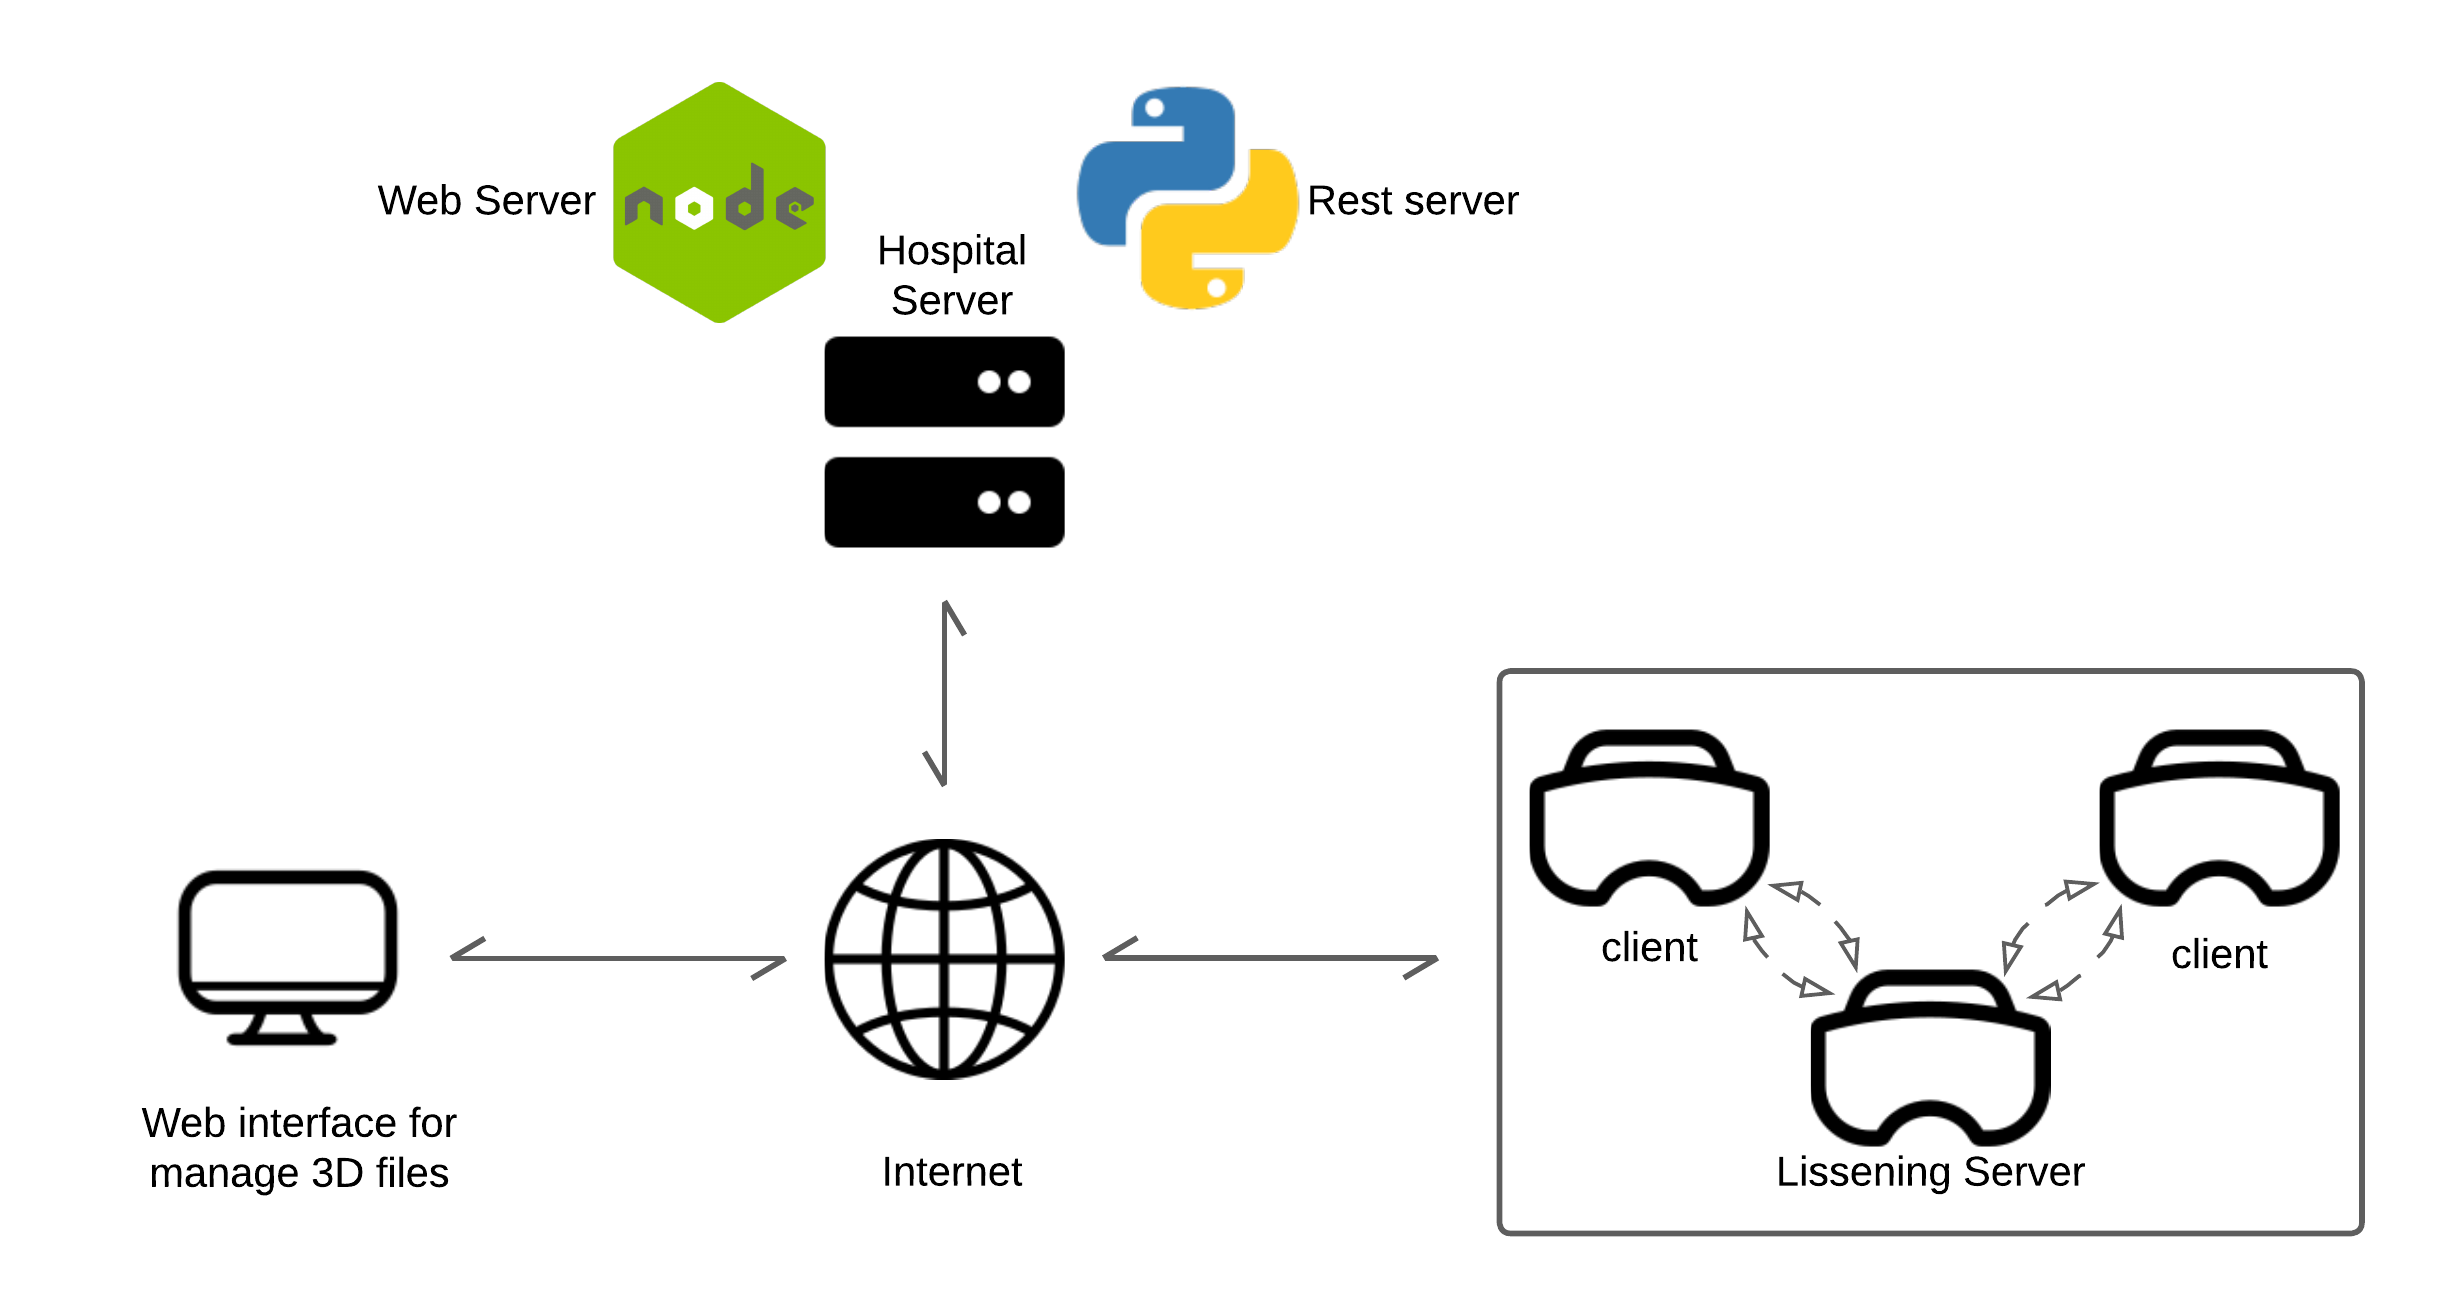
\includegraphics[width=\textwidth]{networkSchema.png}
  \caption{Network Schema}
  \label{fig:NetworkSchema}
\end{figure}


\paragraph{The backend:}
The backend is a simple Python program that functions as a \ac{REST} server, where each 3D model is a resource.
It also manages the multiplayer session by creating the session code, and saves the \ac{IP} address of the listening server.
The library used is called Flask\footnote{\url{https://flask.palletsprojects.com/en/3.0.x/}}, it simply lets you run a function with respect to a \ac{HTTP} response received.

\paragraph{The Web UI:}
The Web \ac{UI} is made with ReactJS, a popular framework for website, the main reason of this choice is for faster development because its community is massive, in fact will be using a UI library called MUI\footnote{\url{https://mui.com/}}
and a 3D library for rendering 3D models called React Three Fiber\footnote{\url{https://r3f.docs.pmnd.rs/getting-started/introduction}}.\\
The main functionality of the Web \ac{UI} will be:
\begin{itemize}
  \item previewing 3D models with the right colors 
  \item upload 3D models
  \item delete 3D models
\end{itemize}


\section{Development environment}
\noindent
It is important to set the right development environment for this project, even if for the Web \ac{UI} and backend it is a standard NodeJS and Python environment, 
it is not that simple for \ac{UE}\\
First the choosing the right version is very important because Meta does not always test all \ac{UE} version, at the start of the developing of the project, the last one was 5.2.1,
we also need Visual Studio with the right components for compile in \texttt{C++}, we could use other text editor, but Visual Studio is the most completed one for unreal.
For other information look at: \cite{UEvisualStudio}
After we set up the basic \ac{UE} environment, we have to pick the right Android studio and \ac{SDK} for building for Android \\
Another important component is the Android \ac{NDK} that enables \ac{UE} to compile native \texttt{C++} code.
But for installing there is a command line tool that \ac{UE} shipped with that can install the right version. 
Because the requirements differ with respect to the version of \ac{UE} for more information look at Epic Games documentation: \cite{UEandroid}.\\
Other than the configuration for Android, we also need to add the right components for building for the Meta Quest 2,
There are two other components useful for developing:
\begin{itemize}
  \item \textbf{MetaXRPlugin:} plugin for: sideload, publish and setting the project for the \ac{HMD}, this component is already implemented in the \ac{UE} fork of META.
  \item \textbf{MetaXRSimulator:} simulator for the \ac{HMD}, this is extremely important because the compile time of the \ac{APK} is slow. The simulator uses a PC instance of the game, and it overlays it.
\end{itemize}
\noindent
For more information look at: \cite{MetaSetup}

